%%%%%%%%%%%%%%%%%%%%%%%%%%%%%%%%%%%%%%%%%
% The Legrand Orange Book
% LaTeX Template
% Version 2.0 (9/2/15)
%
% This template has been downloaded from:
% http://www.LaTeXTemplates.com
%
% Mathias Legrand (legrand.mathias@gmail.com) with modifications by:
% Vel (vel@latextemplates.com)
%
% License:
% CC BY-NC-SA 3.0 (http://creativecommons.org/licenses/by-nc-sa/3.0/)
%
% Compiling this template:
% This template uses biber for its bibliography and makeindex for its index.
% When you first open the template, compile it from the command line with the 
% commands below to make sure your LaTeX distribution is configured correctly:
%
% 1) pdflatex main
% 2) makeindex main.idx -s StyleInd.ist
% 3) biber main
% 4) pdflatex main x 2
%
% After this, when you wish to update the bibliography/index use the appropriate
% command above and make sure to compile with pdflatex several times 
% afterwards to propagate your changes to the document.
%
% This template also uses a number of packages which may need to be
% updated to the newest versions for the template to compile. It is strongly
% recommended you update your LaTeX distribution if you have any
% compilation errors.
%
% Important note:
% Chapter heading images should have a 2:1 width:height ratio,
% e.g. 920px width and 460px height.
%
%%%%%%%%%%%%%%%%%%%%%%%%%%%%%%%%%%%%%%%%%

%----------------------------------------------------------------------------------------
%	PACKAGES AND OTHER DOCUMENT CONFIGURATIONS
%----------------------------------------------------------------------------------------

\documentclass[11pt,fleqn]{book} % Default font size and left-justified equations


\usepackage{mathrsfs}
\usepackage{amsbsy}

%----------------------------------------------------------------------------------------

%fdlkjadlkjdfsal;kjafds;lkjafsd;lkjfsad

%%%%%%%%%%%%%%%%%%%%%%%%%%%%%%%%%%%%%%%%%
% The Legrand Orange Book
% Structural Definitions File
% Version 2.0 (9/2/15)
%
% Original author:
% Mathias Legrand (legrand.mathias@gmail.com) with modifications by:
% Vel (vel@latextemplates.com)
% 
% This file has been downloaded from:
% http://www.LaTeXTemplates.com
%
% License:
% CC BY-NC-SA 3.0 (http://creativecommons.org/licenses/by-nc-sa/3.0/)
%
%%%%%%%%%%%%%%%%%%%%%%%%%%%%%%%%%%%%%%%%%

%----------------------------------------------------------------------------------------
%	VARIOUS REQUIRED PACKAGES AND CONFIGURATIONS
%----------------------------------------------------------------------------------------

\usepackage[top=3cm,bottom=3cm,left=3cm,right=3cm,headsep=10pt,a4paper]{geometry} % Page margins

\usepackage{graphicx} % Required for including pictures
\graphicspath{{Pictures/}} % Specifies the directory where pictures are stored

\usepackage{lipsum} % Inserts dummy text

\usepackage{tikz} % Required for drawing custom shapes

\usepackage[english]{babel} % English language/hyphenation

\usepackage{enumitem} % Customize lists
\setlist{nolistsep} % Reduce spacing between bullet points and numbered lists

\usepackage{booktabs} % Required for nicer horizontal rules in tables

\usepackage{xcolor} % Required for specifying colors by name
\definecolor{ocre}{RGB}{243,102,25} % Define the orange color used for highlighting throughout the book

%----------------------------------------------------------------------------------------
%	FONTS
%----------------------------------------------------------------------------------------

\usepackage{avant} % Use the Avantgarde font for headings
%\usepackage{times} % Use the Times font for headings
\usepackage{mathptmx} % Use the Adobe Times Roman as the default text font together with math symbols from the Sym­bol, Chancery and Com­puter Modern fonts

\usepackage{microtype} % Slightly tweak font spacing for aesthetics
\usepackage[utf8]{inputenc} % Required for including letters with accents
\usepackage[T1]{fontenc} % Use 8-bit encoding that has 256 glyphs

%----------------------------------------------------------------------------------------
%	BIBLIOGRAPHY AND INDEX
%----------------------------------------------------------------------------------------

\usepackage[style=alphabetic,citestyle=numeric,sorting=nyt,sortcites=true,autopunct=true,babel=hyphen,hyperref=true,abbreviate=false,backref=true,backend=biber]{biblatex}
\addbibresource{bibliography.bib} % BibTeX bibliography file
\defbibheading{bibempty}{}

\usepackage{calc} % For simpler calculation - used for spacing the index letter headings correctly
\usepackage{makeidx} % Required to make an index
\makeindex % Tells LaTeX to create the files required for indexing

%----------------------------------------------------------------------------------------
%	MAIN TABLE OF CONTENTS
%----------------------------------------------------------------------------------------

\usepackage{titletoc} % Required for manipulating the table of contents

\contentsmargin{0cm} % Removes the default margin

% Part text styling
\titlecontents{part}[0cm]
{\addvspace{20pt}\centering\large\bfseries}
{}
{}
{}

% Chapter text styling
\titlecontents{chapter}[1.25cm] % Indentation
{\addvspace{12pt}\large\sffamily\bfseries} % Spacing and font options for chapters
{\color{ocre!60}\contentslabel[\Large\thecontentslabel]{1.25cm}\color{ocre}} % Chapter number
{\color{ocre}}  
{\color{ocre!60}\normalsize\;\titlerule*[.5pc]{.}\;\thecontentspage} % Page number

% Section text styling
\titlecontents{section}[1.25cm] % Indentation
{\addvspace{3pt}\sffamily\bfseries} % Spacing and font options for sections
{\contentslabel[\thecontentslabel]{1.25cm}} % Section number
{}
{\hfill\color{black}\thecontentspage} % Page number
[]

% Subsection text styling
\titlecontents{subsection}[1.25cm] % Indentation
{\addvspace{1pt}\sffamily\small} % Spacing and font options for subsections
{\contentslabel[\thecontentslabel]{1.25cm}} % Subsection number
{}
{\ \titlerule*[.5pc]{.}\;\thecontentspage} % Page number
[]

% List of figures
\titlecontents{figure}[0em]
{\addvspace{-5pt}\sffamily}
{\thecontentslabel\hspace*{1em}}
{}
{\ \titlerule*[.5pc]{.}\;\thecontentspage}
[]

% List of tables
\titlecontents{table}[0em]
{\addvspace{-5pt}\sffamily}
{\thecontentslabel\hspace*{1em}}
{}
{\ \titlerule*[.5pc]{.}\;\thecontentspage}
[]

%----------------------------------------------------------------------------------------
%	MINI TABLE OF CONTENTS IN PART HEADS
%----------------------------------------------------------------------------------------

% Chapter text styling
\titlecontents{lchapter}[0em] % Indenting
{\addvspace{15pt}\large\sffamily\bfseries} % Spacing and font options for chapters
{\color{ocre}\contentslabel[\Large\thecontentslabel]{1.25cm}\color{ocre}} % Chapter number
{}  
{\color{ocre}\normalsize\sffamily\bfseries\;\titlerule*[.5pc]{.}\;\thecontentspage} % Page number

% Section text styling
\titlecontents{lsection}[0em] % Indenting
{\sffamily\small} % Spacing and font options for sections
{\contentslabel[\thecontentslabel]{1.25cm}} % Section number
{}
{}

% Subsection text styling
\titlecontents{lsubsection}[.5em] % Indentation
{\normalfont\footnotesize\sffamily} % Font settings
{}
{}
{}

%----------------------------------------------------------------------------------------
%	PAGE HEADERS
%----------------------------------------------------------------------------------------

\usepackage{fancyhdr} % Required for header and footer configuration

\pagestyle{fancy}
\renewcommand{\chaptermark}[1]{\markboth{\sffamily\normalsize\bfseries\chaptername\ \thechapter.\ #1}{}} % Chapter text font settings
\renewcommand{\sectionmark}[1]{\markright{\sffamily\normalsize\thesection\hspace{5pt}#1}{}} % Section text font settings
\fancyhf{} \fancyhead[LE,RO]{\sffamily\normalsize\thepage} % Font setting for the page number in the header
\fancyhead[LO]{\rightmark} % Print the nearest section name on the left side of odd pages
\fancyhead[RE]{\leftmark} % Print the current chapter name on the right side of even pages
\renewcommand{\headrulewidth}{0.5pt} % Width of the rule under the header
\addtolength{\headheight}{2.5pt} % Increase the spacing around the header slightly
\renewcommand{\footrulewidth}{0pt} % Removes the rule in the footer
\fancypagestyle{plain}{\fancyhead{}\renewcommand{\headrulewidth}{0pt}} % Style for when a plain pagestyle is specified

% Removes the header from odd empty pages at the end of chapters
\makeatletter
\renewcommand{\cleardoublepage}{
\clearpage\ifodd\c@page\else
\hbox{}
\vspace*{\fill}
\thispagestyle{empty}
\newpage
\fi}

%----------------------------------------------------------------------------------------
%	THEOREM STYLES
%----------------------------------------------------------------------------------------

\usepackage{amsmath,amsfonts,amssymb,amsthm} % For math equations, theorems, symbols, etc

\newcommand{\intoo}[2]{\mathopen{]}#1\,;#2\mathclose{[}}
\newcommand{\ud}{\mathop{\mathrm{{}d}}\mathopen{}}
\newcommand{\intff}[2]{\mathopen{[}#1\,;#2\mathclose{]}}
\newtheorem{notation}{Notation}[chapter]

% Boxed/framed environments
\newtheoremstyle{ocrenumbox}% % Theorem style name
{0pt}% Space above
{0pt}% Space below
{\normalfont}% % Body font
{}% Indent amount
{\small\bf\sffamily\color{ocre}}% % Theorem head font
{\;}% Punctuation after theorem head
{0.25em}% Space after theorem head
{\small\sffamily\color{ocre}\thmname{#1}\nobreakspace\thmnumber{\@ifnotempty{#1}{}\@upn{#2}}% Theorem text (e.g. Theorem 2.1)
\thmnote{\nobreakspace\the\thm@notefont\sffamily\bfseries\color{black}---\nobreakspace#3.}} % Optional theorem note
\renewcommand{\qedsymbol}{$\blacksquare$}% Optional qed square

\newtheoremstyle{blacknumex}% Theorem style name
{5pt}% Space above
{5pt}% Space below
{\normalfont}% Body font
{} % Indent amount
{\small\bf\sffamily}% Theorem head font
{\;}% Punctuation after theorem head
{0.25em}% Space after theorem head
{\small\sffamily{\tiny\ensuremath{\blacksquare}}\nobreakspace\thmname{#1}\nobreakspace\thmnumber{\@ifnotempty{#1}{}\@upn{#2}}% Theorem text (e.g. Theorem 2.1)
\thmnote{\nobreakspace\the\thm@notefont\sffamily\bfseries---\nobreakspace#3.}}% Optional theorem note

\newtheoremstyle{blacknumbox} % Theorem style name
{0pt}% Space above
{0pt}% Space below
{\normalfont}% Body font
{}% Indent amount
{\small\bf\sffamily}% Theorem head font
{\;}% Punctuation after theorem head
{0.25em}% Space after theorem head
{\small\sffamily\thmname{#1}\nobreakspace\thmnumber{\@ifnotempty{#1}{}\@upn{#2}}% Theorem text (e.g. Theorem 2.1)
\thmnote{\nobreakspace\the\thm@notefont\sffamily\bfseries---\nobreakspace#3.}}% Optional theorem note

% Non-boxed/non-framed environments
\newtheoremstyle{ocrenum}% % Theorem style name
{5pt}% Space above
{5pt}% Space below
{\normalfont}% % Body font
{}% Indent amount
{\small\bf\sffamily\color{ocre}}% % Theorem head font
{\;}% Punctuation after theorem head
{0.25em}% Space after theorem head
{\small\sffamily\color{ocre}\thmname{#1}\nobreakspace\thmnumber{\@ifnotempty{#1}{}\@upn{#2}}% Theorem text (e.g. Theorem 2.1)
\thmnote{\nobreakspace\the\thm@notefont\sffamily\bfseries\color{black}---\nobreakspace#3.}} % Optional theorem note
\renewcommand{\qedsymbol}{$\blacksquare$}% Optional qed square
\makeatother

% Defines the theorem text style for each type of theorem to one of the three styles above
\newcounter{dummy} 
\numberwithin{dummy}{section}
\theoremstyle{ocrenumbox}
\newtheorem{theoremeT}[dummy]{Theorem}
\newtheorem{problem}{Problem}[chapter]
\newtheorem{exerciseT}{Exercise}[chapter]
\theoremstyle{blacknumex}
\newtheorem{exampleT}{Example}[chapter]
\theoremstyle{blacknumbox}
\newtheorem{vocabulary}{Vocabulary}[chapter]
\newtheorem{definitionT}{Definition}[section]
\newtheorem{corollaryT}[dummy]{Corollary}
\theoremstyle{ocrenum}
\newtheorem{proposition}[dummy]{Proposition}

%----------------------------------------------------------------------------------------
%	DEFINITION OF COLORED BOXES
%----------------------------------------------------------------------------------------

\RequirePackage[framemethod=default]{mdframed} % Required for creating the theorem, definition, exercise and corollary boxes

% Theorem box
\newmdenv[skipabove=7pt,
skipbelow=7pt,
backgroundcolor=black!5,
linecolor=ocre,
innerleftmargin=5pt,
innerrightmargin=5pt,
innertopmargin=5pt,
leftmargin=0cm,
rightmargin=0cm,
innerbottommargin=5pt]{tBox}

% Exercise box	  
\newmdenv[skipabove=7pt,
skipbelow=7pt,
rightline=false,
leftline=true,
topline=false,
bottomline=false,
backgroundcolor=ocre!10,
linecolor=ocre,
innerleftmargin=5pt,
innerrightmargin=5pt,
innertopmargin=5pt,
innerbottommargin=5pt,
leftmargin=0cm,
rightmargin=0cm,
linewidth=4pt]{eBox}	

% Definition box
\newmdenv[skipabove=7pt,
skipbelow=7pt,
rightline=false,
leftline=true,
topline=false,
bottomline=false,
linecolor=ocre,
innerleftmargin=5pt,
innerrightmargin=5pt,
innertopmargin=0pt,
leftmargin=0cm,
rightmargin=0cm,
linewidth=4pt,
innerbottommargin=0pt]{dBox}	

% Corollary box
\newmdenv[skipabove=7pt,
skipbelow=7pt,
rightline=false,
leftline=true,
topline=false,
bottomline=false,
linecolor=gray,
backgroundcolor=black!5,
innerleftmargin=5pt,
innerrightmargin=5pt,
innertopmargin=5pt,
leftmargin=0cm,
rightmargin=0cm,
linewidth=4pt,
innerbottommargin=5pt]{cBox}

% Creates an environment for each type of theorem and assigns it a theorem text style from the "Theorem Styles" section above and a colored box from above
\newenvironment{theorem}{\begin{tBox}\begin{theoremeT}}{\end{theoremeT}\end{tBox}}
\newenvironment{exercise}{\begin{eBox}\begin{exerciseT}}{\hfill{\color{ocre}\tiny\ensuremath{\blacksquare}}\end{exerciseT}\end{eBox}}				  
\newenvironment{definition}{\begin{dBox}\begin{definitionT}}{\end{definitionT}\end{dBox}}	
\newenvironment{example}{\begin{exampleT}}{\hfill{\tiny\ensuremath{\blacksquare}}\end{exampleT}}		
\newenvironment{corollary}{\begin{cBox}\begin{corollaryT}}{\end{corollaryT}\end{cBox}}	

%----------------------------------------------------------------------------------------
%	REMARK ENVIRONMENT
%----------------------------------------------------------------------------------------

\newenvironment{remark}{\par\vspace{10pt}\small % Vertical white space above the remark and smaller font size
\begin{list}{}{
\leftmargin=35pt % Indentation on the left
\rightmargin=25pt}\item\ignorespaces % Indentation on the right
\makebox[-2.5pt]{\begin{tikzpicture}[overlay]
\node[draw=ocre!60,line width=1pt,circle,fill=ocre!25,font=\sffamily\bfseries,inner sep=2pt,outer sep=0pt] at (-15pt,0pt){\textcolor{ocre}{R}};\end{tikzpicture}} % Orange R in a circle
\advance\baselineskip -1pt}{\end{list}\vskip5pt} % Tighter line spacing and white space after remark

%----------------------------------------------------------------------------------------
%	SECTION NUMBERING IN THE MARGIN
%----------------------------------------------------------------------------------------

\makeatletter
\renewcommand{\@seccntformat}[1]{\llap{\textcolor{ocre}{\csname the#1\endcsname}\hspace{1em}}}                    
\renewcommand{\section}{\@startsection{section}{1}{\z@}
{-4ex \@plus -1ex \@minus -.4ex}
{1ex \@plus.2ex }
{\normalfont\large\sffamily\bfseries}}
\renewcommand{\subsection}{\@startsection {subsection}{2}{\z@}
{-3ex \@plus -0.1ex \@minus -.4ex}
{0.5ex \@plus.2ex }
{\normalfont\sffamily\bfseries}}
\renewcommand{\subsubsection}{\@startsection {subsubsection}{3}{\z@}
{-2ex \@plus -0.1ex \@minus -.2ex}
{.2ex \@plus.2ex }
{\normalfont\small\sffamily\bfseries}}                        
\renewcommand\paragraph{\@startsection{paragraph}{4}{\z@}
{-2ex \@plus-.2ex \@minus .2ex}
{.1ex}
{\normalfont\small\sffamily\bfseries}}

%----------------------------------------------------------------------------------------
%	PART HEADINGS
%----------------------------------------------------------------------------------------

% numbered part in the table of contents
\newcommand{\@mypartnumtocformat}[2]{%
\setlength\fboxsep{0pt}%
\noindent\colorbox{ocre!20}{\strut\parbox[c][.7cm]{\ecart}{\color{ocre!70}\Large\sffamily\bfseries\centering#1}}\hskip\esp\colorbox{ocre!40}{\strut\parbox[c][.7cm]{\linewidth-\ecart-\esp}{\Large\sffamily\centering#2}}}%
%%%%%%%%%%%%%%%%%%%%%%%%%%%%%%%%%%
% unnumbered part in the table of contents
\newcommand{\@myparttocformat}[1]{%
\setlength\fboxsep{0pt}%
\noindent\colorbox{ocre!40}{\strut\parbox[c][.7cm]{\linewidth}{\Large\sffamily\centering#1}}}%
%%%%%%%%%%%%%%%%%%%%%%%%%%%%%%%%%%
\newlength\esp
\setlength\esp{4pt}
\newlength\ecart
\setlength\ecart{1.2cm-\esp}
\newcommand{\thepartimage}{}%
\newcommand{\partimage}[1]{\renewcommand{\thepartimage}{#1}}%
\def\@part[#1]#2{%
\ifnum \c@secnumdepth >-2\relax%
\refstepcounter{part}%
\addcontentsline{toc}{part}{\texorpdfstring{\protect\@mypartnumtocformat{\thepart}{#1}}{\partname~\thepart\ ---\ #1}}
\else%
\addcontentsline{toc}{part}{\texorpdfstring{\protect\@myparttocformat{#1}}{#1}}%
\fi%
\startcontents%
\markboth{}{}%
{\thispagestyle{empty}%
\begin{tikzpicture}[remember picture,overlay]%
\node at (current page.north west){\begin{tikzpicture}[remember picture,overlay]%	
\fill[ocre!20](0cm,0cm) rectangle (\paperwidth,-\paperheight);
\node[anchor=north] at (4cm,-3.25cm){\color{ocre!40}\fontsize{220}{100}\sffamily\bfseries\@Roman\c@part}; 
\node[anchor=south east] at (\paperwidth-1cm,-\paperheight+1cm){\parbox[t][][t]{8.5cm}{
\printcontents{l}{0}{\setcounter{tocdepth}{1}}%
}};
\node[anchor=north east] at (\paperwidth-1.5cm,-3.25cm){\parbox[t][][t]{15cm}{\strut\raggedleft\color{white}\fontsize{30}{30}\sffamily\bfseries#2}};
\end{tikzpicture}};
\end{tikzpicture}}%
\@endpart}
\def\@spart#1{%
\startcontents%
\phantomsection
{\thispagestyle{empty}%
\begin{tikzpicture}[remember picture,overlay]%
\node at (current page.north west){\begin{tikzpicture}[remember picture,overlay]%	
\fill[ocre!20](0cm,0cm) rectangle (\paperwidth,-\paperheight);
\node[anchor=north east] at (\paperwidth-1.5cm,-3.25cm){\parbox[t][][t]{15cm}{\strut\raggedleft\color{white}\fontsize{30}{30}\sffamily\bfseries#1}};
\end{tikzpicture}};
\end{tikzpicture}}
\addcontentsline{toc}{part}{\texorpdfstring{%
\setlength\fboxsep{0pt}%
\noindent\protect\colorbox{ocre!40}{\strut\protect\parbox[c][.7cm]{\linewidth}{\Large\sffamily\protect\centering #1\quad\mbox{}}}}{#1}}%
\@endpart}
\def\@endpart{\vfil\newpage
\if@twoside
\if@openright
\null
\thispagestyle{empty}%
\newpage
\fi
\fi
\if@tempswa
\twocolumn
\fi}

%----------------------------------------------------------------------------------------
%	CHAPTER HEADINGS
%----------------------------------------------------------------------------------------

\newcommand{\thechapterimage}{}%
\newcommand{\chapterimage}[1]{\renewcommand{\thechapterimage}{#1}}%
\def\@makechapterhead#1{%
{\parindent \z@ \raggedright \normalfont
\ifnum \c@secnumdepth >\m@ne
\if@mainmatter
\begin{tikzpicture}[remember picture,overlay]
\node at (current page.north west)
{\begin{tikzpicture}[remember picture,overlay]
\node[anchor=north west,inner sep=0pt] at (0,0) {\includegraphics[width=\paperwidth]{\thechapterimage}};
\draw[anchor=west] (\Gm@lmargin,-9cm) node [line width=2pt,rounded corners=15pt,draw=ocre,fill=white,fill opacity=0.5,inner sep=15pt]{\strut\makebox[22cm]{}};
\draw[anchor=west] (\Gm@lmargin+.3cm,-9cm) node {\huge\sffamily\bfseries\color{black}\thechapter. #1\strut};
\end{tikzpicture}};
\end{tikzpicture}
\else
\begin{tikzpicture}[remember picture,overlay]
\node at (current page.north west)
{\begin{tikzpicture}[remember picture,overlay]
\node[anchor=north west,inner sep=0pt] at (0,0) {\includegraphics[width=\paperwidth]{\thechapterimage}};
\draw[anchor=west] (\Gm@lmargin,-9cm) node [line width=2pt,rounded corners=15pt,draw=ocre,fill=white,fill opacity=0.5,inner sep=15pt]{\strut\makebox[22cm]{}};
\draw[anchor=west] (\Gm@lmargin+.3cm,-9cm) node {\huge\sffamily\bfseries\color{black}#1\strut};
\end{tikzpicture}};
\end{tikzpicture}
\fi\fi\par\vspace*{270\p@}}}

%-------------------------------------------

\def\@makeschapterhead#1{%
\begin{tikzpicture}[remember picture,overlay]
\node at (current page.north west)
{\begin{tikzpicture}[remember picture,overlay]
\node[anchor=north west,inner sep=0pt] at (0,0) {\includegraphics[width=\paperwidth]{\thechapterimage}};
\draw[anchor=west] (\Gm@lmargin,-9cm) node [line width=2pt,rounded corners=15pt,draw=ocre,fill=white,fill opacity=0.5,inner sep=15pt]{\strut\makebox[22cm]{}};
\draw[anchor=west] (\Gm@lmargin+.3cm,-9cm) node {\huge\sffamily\bfseries\color{black}#1\strut};
\end{tikzpicture}};
\end{tikzpicture}
\par\vspace*{270\p@}}
\makeatother

%----------------------------------------------------------------------------------------
%	HYPERLINKS IN THE DOCUMENTS
%----------------------------------------------------------------------------------------

\usepackage{hyperref}
\hypersetup{hidelinks,backref=true,pagebackref=true,hyperindex=true,colorlinks=false,breaklinks=true,urlcolor= ocre,bookmarks=true,bookmarksopen=false,pdftitle={Title},pdfauthor={Author}}
\usepackage{bookmark}
\bookmarksetup{
open,
numbered,
addtohook={%
\ifnum\bookmarkget{level}=0 % chapter
\bookmarksetup{bold}%
\fi
\ifnum\bookmarkget{level}=-1 % part
\bookmarksetup{color=ocre,bold}%
\fi
}
}
 % Insert the commands.tex file which contains the majority of the structure behind the template

\begin{document}

%----------------------------------------------------------------------------------------
%	TITLE PAGE
%----------------------------------------------------------------------------------------

\begingroup
\thispagestyle{empty}
\begin{tikzpicture}[remember picture,overlay]
\coordinate [below=12cm] (midpoint) at (current page.north);
\node at (current page.north west)
{\begin{tikzpicture}[remember picture,overlay]
\node[anchor=north west,inner sep=0pt] at (0,0) {
\includegraphics[width=\paperwidth]{background}}; % Background image
\draw[anchor=north] (midpoint) node [fill=ocre!30!white,fill opacity=0.6,text opacity=1,inner sep=1cm]{\Huge\centering\bfseries\sffamily\parbox[c][][t]{\paperwidth}{\centering Probability Theroy based on Measure Theory\\[15pt] % Book title
{\Large STAT 517}\\[20pt] % Subtitle
{\huge Dr. John Smith}}}; % Author name
\end{tikzpicture}};
\end{tikzpicture}
\vfill
\endgroup

%----------------------------------------------------------------------------------------
%	COPYRIGHT PAGE
%----------------------------------------------------------------------------------------

\newpage
~\vfill
\thispagestyle{empty}

\noindent Copyright \copyright\ 2013 John Smith\\ % Copyright notice

\noindent \textsc{Published by Publisher}\\ % Publisher

\noindent \textsc{book-website.com}\\ % URL

\noindent Licensed under the Creative Commons Attribution-NonCommercial 3.0 Unported License (the ``License''). You may not use this file except in compliance with the License. You may obtain a copy of the License at \url{http://creativecommons.org/licenses/by-nc/3.0}. Unless required by applicable law or agreed to in writing, software distributed under the License is distributed on an \textsc{``as is'' basis, without warranties or conditions of any kind}, either express or implied. See the License for the specific language governing permissions and limitations under the License.\\ % License information

\noindent \textit{First printing, March 2013} % Printing/edition date

%----------------------------------------------------------------------------------------
%	TABLE OF CONTENTS
%----------------------------------------------------------------------------------------

\chapterimage{chapter_head_1.pdf} % Table of contents heading image

\pagestyle{empty} % No headers

\tableofcontents % Print the table of contents itself

\cleardoublepage % Forces the first chapter to start on an odd page so it's on the right

\pagestyle{fancy} % Print headers again

%----------------------------------------------------------------------------------------
%	PART
%----------------------------------------------------------------------------------------

\part{Part One}

%----------------------------------------------------------------------------------------
%	CHAPTER 1
%----------------------------------------------------------------------------------------

\chapterimage{chapter_head_2.pdf} % Chapter heading image

\chapter{Probability Measure}

\section{Probability on a Field}\index{Probability on a Field}
% Section Two in Billingsly

\begin{definition}[$\Omega$] Non emtpy set. 
	
\end{definition}

\begin{definition}[Paving] A collection of a subset of $\Omega$ is a paving. 
	
\end{definition}

\begin{definition}[Field] A \textbf{field} $\mathscr{F}$ is a paving satisfying
	\begin{enumerate}[label = (\roman*)]
		\item $\Omega \in \mathscr{F}$
		\item $A \in \mathscr{F} \Rightarrow A^C \in \mathscr{F}$
		\item $A, B, \in \mathscr{F}, \Rightarrow A \cup B \in \mathscr{F}$
	\end{enumerate}
	
\end{definition}

\textbf{Derived Properties about a Field }

\begin{itemize}
	\item $\emptyset \in \mathscr{F}$ 
		(by (i) and (ii): 
		\begin{align*}
			\Omega \in \mathscr{F} &\Rightarrow \Omega^C \in \mathscr{F}\\
			&\Rightarrow \emptyset \in \mathscr{F})
		\end{align*}
			
	\item (i) can be replaced by "$\mathscr{R}$ is nonempty" because,\\ 
		Let $A \in \mathscr{F}, $
			\begin{align*}
				&\Rightarrow A^c \in \mathscr{F}\\
			&\Rightarrow A^C \cup A \in \mathscr{F}\\
			&\Rightarrow \Omega \in \mathscr{F}\\
			\end{align*}
			
	\item $A \in \mathscr{F}, B \in \mathscr{F}, \Rightarrow, A\cap B \in \mathscr{F}$ 
	because, \\
		\begin{align*}
		&(A\cap B)^C = A^C \cup B^C (DeMorgan's Law)\\
		&A \cap B = (A^C \cup B^C)^C	
		\end{align*}
		

	\item $A_1, \dots, A_m \in \mathscr{F} \Rightarrow A_1 \cup, \dots, \cup A_m \in \mathscr{F} $ (mathematical induction)
	\item$A_1, \dots, A_m \in \mathscr{F} \Rightarrow A_1 \cap, \dots, \cap A_m \in \mathscr{F} $ 
\end{itemize}



\begin{definition}[$\sigma$-Field] Similar to the definition of a field except for (iii). A paving satisfying 
	\begin{enumerate}[label = (\roman*)]
		\item $\Omega \in \mathscr{F}$
		\item $A \in \mathscr{F} \Rightarrow A^C \in \mathscr{F}$
		\item $A_1 \in \mathscr{F}, \dots, A_m \in \mathscr{F} $\\ $\displaystyle\cup_{k=1}^m A_k \in \mathscr{F}$ (finite additvity)
	\end{enumerate}
\vspace{5mm}

If we replace (iii) from before by (iii') here:

For $A_1 \in \mathscr{F}, \dots, A_m \in \mathscr{F}$ 

$$\cup_{k=1}^\infty A_k \in \mathscr{F}$$

then $\mathscr{F}$ is called a $\sigma$\textbf{-field}. 
\end{definition}


	


\textbf{Derived Facts}

\begin{itemize}
	\item Again, (i) can be repalced by $\mathscr{F}$ no empty, 
				(iii) can be replaced  $A_1 \in \mathscr{F}, \dots, A_m \in \mathscr{F} $
\end{itemize}

\begin{example}
	$\Omega = (0, 1]$ (from now on all intervals are left open, right closed)\\

	\begin{remark}
		Recall that $\sigma$-fields are generated by fields. Fancy scripts denote a $\sigma$-field. Fancy scripts with a zero subscript denote a field.
	\end{remark}

	$\mathscr{B}_0$ is the collection of all finite union of disjoint intervals. Asside: something that we can consider easily, but computers cannot. (e.g. think of all stars, etc)

	\begin{figure}[h]
	\centering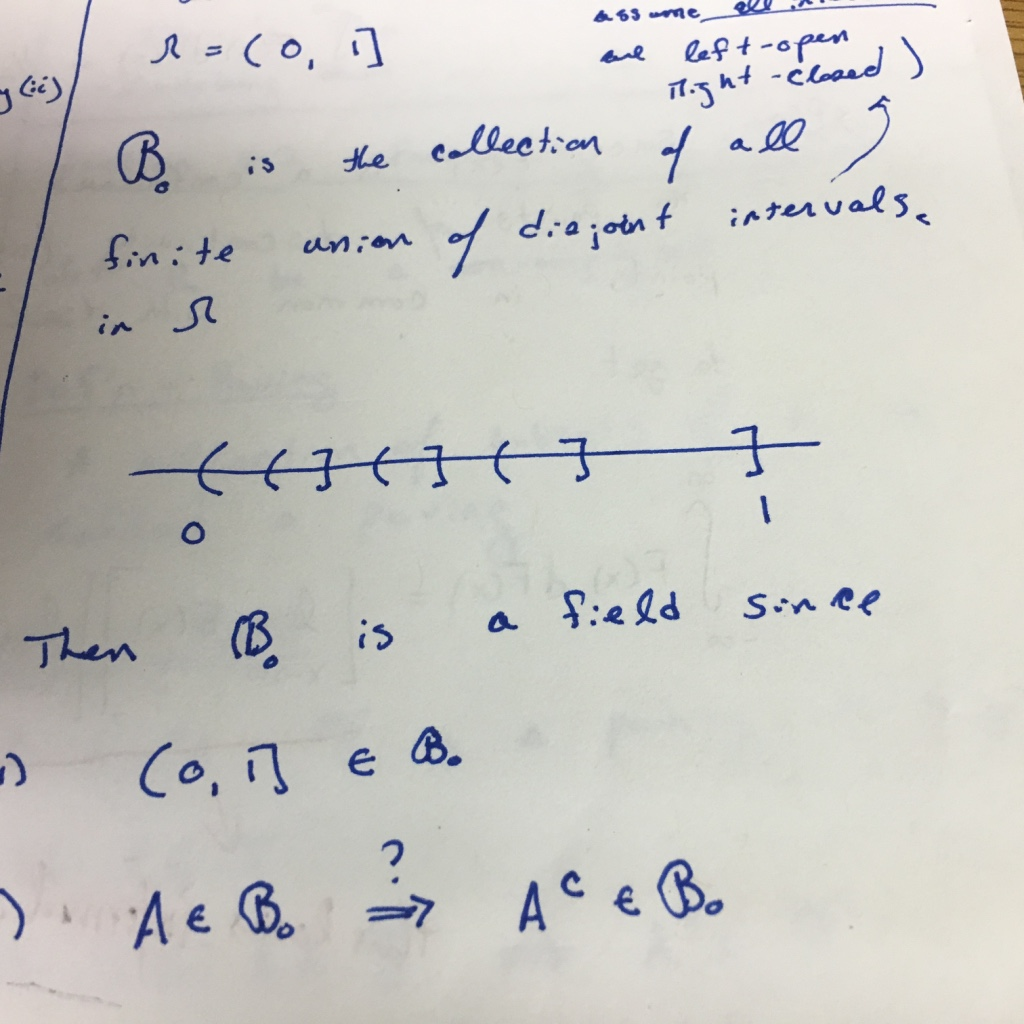
\includegraphics[scale=0.15]{notes1.jpg}
	\caption{Finite unioin of three disjoint intervals.}
	\end{figure}

	Then $\mathscr{B}_0$ is a field. 

	\begin{enumerate}[label = (\roman*)]
		\item (0, 1] $\in \mathscr{B}_0$
		\item $A \in \mathscr{B}_0 \Rightarrow A^c \in \mathscr{B}_0$ 
		\begin{figure}[h]
		\centering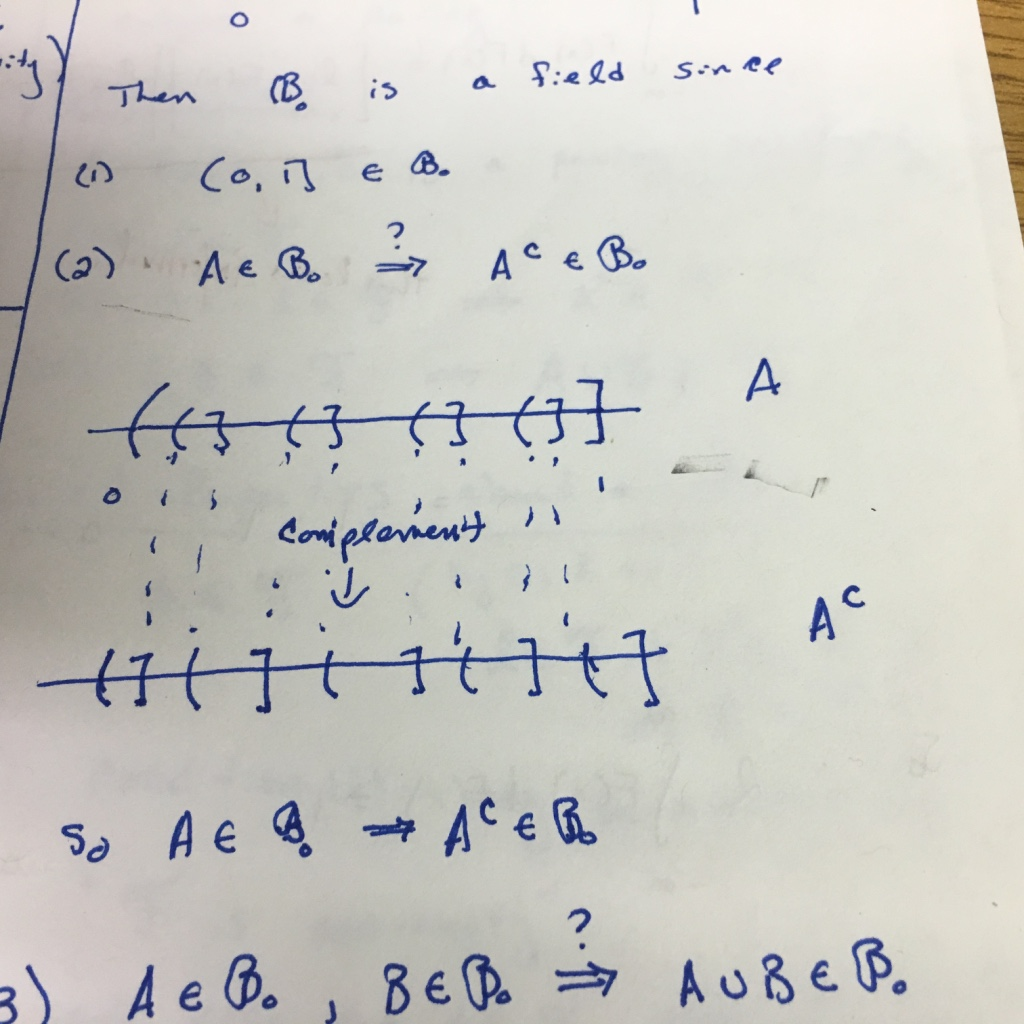
\includegraphics[scale=0.15]{notes2.jpg}
		\caption{A and complement of A.}
		\end{figure}

		\item $A \in \mathscr{B}_o, B \in \mathscr{B}_o \Rightarrow A \cup B \in \mathscr{B}_o$ 

		\begin{figure}[h]
		\centering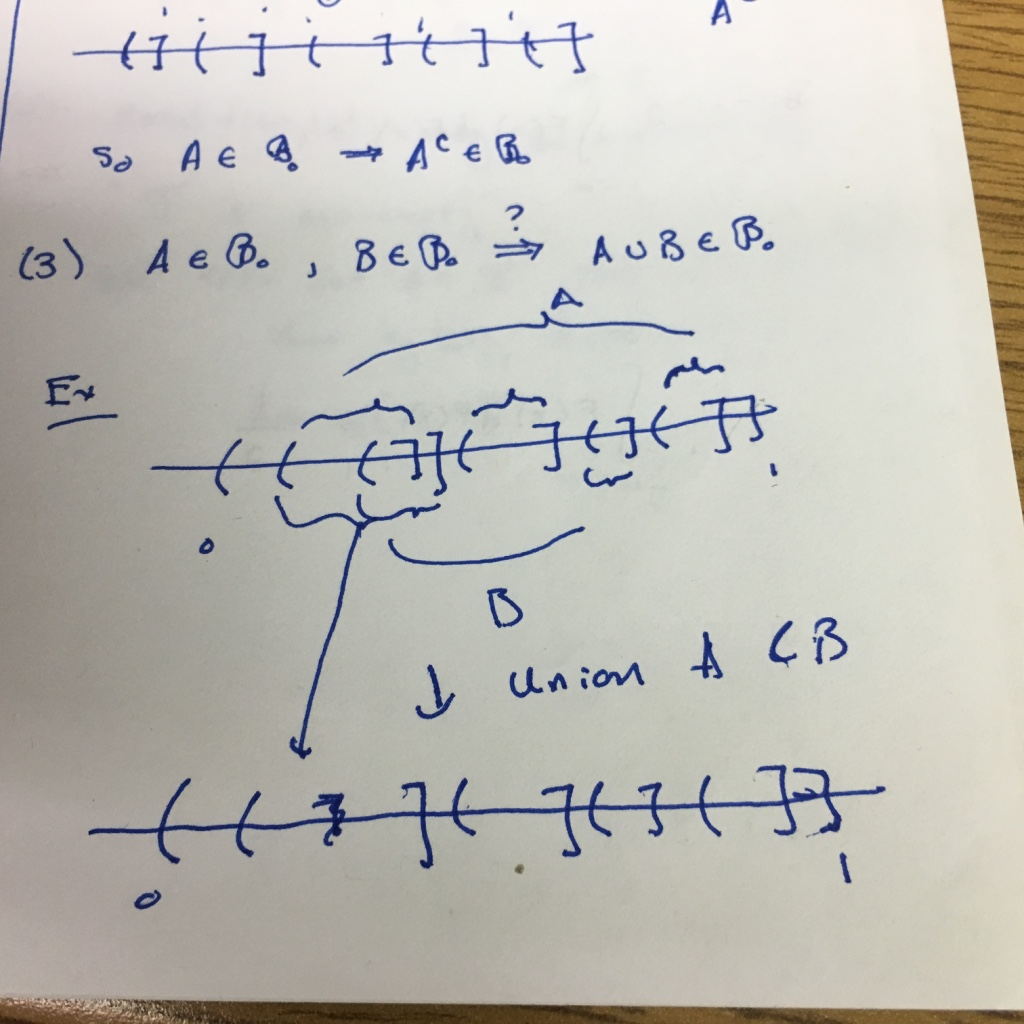
\includegraphics[scale=0.15]{notes3.jpg}
		\caption{Union of A and B is still in $\mathscr{B}_o$}
		\end{figure}

	\end{enumerate}


\end{example}


\textbf{Wednesday August 24}

$\mathscr{B}_0 = $ collection of finite unions of disjoin subintervals of (0, 1]. Is a field. \\
\\

\begin{definition}[Power Set]
	A $\sigma$-field is generated by a paving of power set. Let $\Omega$ be a set. The collection of all subsets of $\Omega$ is the power set written as $2^\Omega$.
\end{definition}

\begin{remark}
	Where does this notation come from?

Consider ths case where $\Omega$ is finite

$$\Omega = \{\omega_1, \dots, \omega_n \} $$

Total number of subsets of $\Omega$. 

$\emptyset, 1$ element sets, 2-element sets, $\dots$, n-element ests.

$$() + () + \dots + = (1+1)^n$$

$\#(\mathscr{F})  = 2^{\# \Omega}$, so it seems reasonable to denote $\mathscr{F} = 2^\Omega$. 

It is also easy to show that $2^\Omega$ is a $\sigma$-field. (The largest, even. The smallest: $\{\emptyset, \Omega\}$ which is also a $\sigma$-field.)

$$\{\emptyset, \Omega\} \subseteq \sigma\text{-field} \subseteq 2^\Omega$$ 
\end{remark}

It turns out we can extend notion of lenght from $\mathscr{B}_0$ to $\sigma$-field generated by $\mathscr{B}_o$. \\
\\
Now, let $\mathscr{A}$ be a nonempty paving of $\Omega$. We define 
$$\sigma(\mathscr{A}) = \cap \{\mathscr{B} \subseteq 2^\Omega: \mathscr{B}\text{ is a }\sigma\text{-field}, \mathscr{A} \subseteq \mathscr{B}\} $$

OR rather, the \textit{intersection} of all $\sigma$-fields that contains $\mathscr{A}$. \\
\\
Let 
$$\mathbb{F}(\mathscr{A}) = \{\mathscr{B} \subseteq 2^\Omega: \mathscr{B} \text{ is a } \sigma\text{-field, } \mathscr{B} \supseteq \mathscr{A} \}$$

Then, 
$$\sigma(\mathscr{A}) = \cap \mathscr{B}$$
$$\mathscr{B} \in \mathbb{F}(\mathscr{A}) $$

\textbf{Derived Facts}

$\mathbb{F}(\mathscr{A})$ is nonempty. For example, $2^\Omega$ is a $\sigma$-field and $2^\Omega \supseteq \mathscr{A}$. 

$\cap B$ is a $\sigma$-field. ($B \in \mathbb{F}(\mathscr{A})$)

\begin{remark}
	Get notes about notation/levels.
\end{remark}

\begin{proof} We will prove that indeed $\sigma(\mathscr{A})$ is a $\sigma$ -field. Recall that we have three conditions above for $\sigma$-field.\\
\\
	\begin{enumerate}[label = (\roman*)]
		\item $$\Omega \in \sigma(\mathscr{A})$$ 
			$$\Omega \in \cap_{B \in \mathbb{F}(\mathscr{A})} B $$
			Because: B is $\sigma$-field, $A \in B$, $\forall B \in \mathbb{F}(\mathscr{A})$.
		\item 
			% \begin{align*}
			% 	A \in \cap B &\Rightarrow A \in B \forall B \in\mathbb{F}(\mathscr{A})\\
			% 	&\Rightarrow A^C \in B , \forall B  \in \mathbb{F}(\mathscr{A})\\ 
			% 	&\Rightarrow A^C \in \cap_{B \in \mathbb{F}(\mathscr{A}) B\\
			% \end{align*}

		\item $A_1, \dots, \in \cap_{B \in \mathbb{F}(\mathscr{A})} B, \forall  B  \in \mathbb{F}(\mathscr{A})$

		$\Rightarrow \cup^\infty_{n =1} A_n \in B, \forall B \in \mathbb{F}(\mathscr{A})$

	\end{enumerate}

	So, $\sigma(\mathscr{A}$ is a $\sigma$-field, we call it the $\sigma$-field, generated by $\mathscr{B}_o$. We know how tot assign lenth to members of $\mathscr{B}_o$, we now show the assignment can be extended to $\sigma(\mathscr{B}_o)$ 


\end{proof}

\begin{example}
	 Let $\mathscr{I}$ be the collection of \textit{all} subintervals of (0,1].\\
	\\
	 Note that $\mathscr{I}$ is a smaller collection than $\mathscr{B}_0$ since $\mathscr{B}_0$ can have numerous different combinations of the sets. 

	 Let

	$$\mathscr{B} = \sigma(\mathscr{I})$$. 

	This is a Borel-$\sigma$-field. (a member of $\mathscr{B}$ in Borel set.)

	It turns out

	$$\sigma(\mathscr{I}) = \sigma(\mathscr{B}_o)  $$

This is because $\sigma(\mathscr{I})$ is a $\sigma$-field. 

So, 
	\begin{align*}
		\sigma(\mathscr{I}) &\supseteq \mathscr{B}_o\\
		\sigma(\mathscr{I}) &\supseteq \sigma(\mathscr{B}_o)
	\end{align*}

Also, 
\begin{align*}
		\mathscr{I} &\subseteq \mathscr{B}_o\\
		\sigma(\mathscr{I}) &\subseteq \sigma(\mathscr{B}_o)
	\end{align*} 

Thus, 
\begin{align*}
	\sigma(\mathscr{I}) &= \sigma(\mathscr{B}_o)
\end{align*}
\end{example}




\begin{definition}[Probability Measure]

Probablity measures on field. Suppose $\mathscr{F}$ is a field on a nonempy set $\Omega$. A probability measure is a function $P:\mathscr{F} \rightarrow \mathbb{R}$. 

\begin{enumerate}[label = (\roman*)]
	\item $0 \leq P(A) \leq 1, \forall A \in \mathscr{F}$
	\item $P(\emptyset) = 0$, $P(\Omega) = 1$
	\item If $A_1, \dots$ are disjoint emembers of $\mathscr{F}$ and $\cup A_n \in \mathscr{F}$ then we have countable additivity:

	$$P (\cup A_n) = \displaystyle\sum^\infty_{n=1} P(A_N) $$
\end{enumerate}

\begin{remark}
	Note that (iii) also implies finite additivity. Prove by adding infinite empty sets on end. 
\end{remark}

	
\end{definition}


If $\Omega$ is nonempty set. 
And $\mathscr{F}$ is a $\sigma$-field on $\Omega$.
And P is a probability measure on $\mathscr{F}$.

Then ($\Omega, \mathscr{F}, P$) is called a \textbf{probability space.}

And ($\Omega, \mathscr{F}$) is called a \textbf{measurable space.}


\begin{remark}
	If $A \subseteq B$, then $P(A) \leq P(B)$. This is because we may write B as

	$$B = A \cup (B\setminus A) $$
\end{remark}

\begin{remark}
	$$P(A) + P(B) = P(A\cup B) + P(A \cap B)$$


\end{remark}

\textbf{Friday August 26}
\\

Recall, 

Probability measure on a field, $\mathscr{F}_0$.

\begin{itemize}
	\item $P(A) + P(B) = P(A\cup B) + P(A \cap B)$

	% GET VINN DIAGRAM
	\begin{itemize}
		\item $P(A) = P(AB^C) + P(A B)$
		\item $P(B) = P(B A^C) + P(AB)$
		\item $P(A) + P(B) = P(AB^C) + P(BA^C) + 2P(AB)$
		\item $P(A \cup B) = P(AB^C) + P(BA^C) + P(AB)$ 
	\end{itemize}
	
	\item $P(A \cup B) = P(A) + P(B) - P(AB)$
		By induction, we can prove if $A_1, \dots A_n$,

		$$P(\displaystyle \cup^n_{k=1} A_k) = \displaystyle \sum^n_{k=1} P(A_k) - \displaystyle \sum_{i<j} P(A_iA_j) +
		\displaystyle \sum_{i<j<k} A_iA_j) + \dots + (-1)^{n+1} P(A_1, \dots, A_n)  $$

		Inclusion- Exclusion Formula

	\item If $A_1, \dots A_n \in \mathscr{F}$,

		$$B_1 = A_1 $$
		$$B_2 = A_2 \setminus A_1$$
		$$\vdots $$

		Then, 
		$$\displaystyle \cup^n_{k=1} A_k = \displaystyle \cup^n_{k=1} B_k $$

		but the $B_i$ are disjoint. Also $A_K \subseteq B_k \forall k=1, \dots, n$.

		$$ P(\displaystyle \cup^n_{k=1} A_k) = P(\displaystyle \cup^n_{k=1} B_k) = \displaystyle \sum^n_{k=1} B_k \leq \displaystyle \sum^n_{k=1} A_k$$

		Thus, $P(\displaystyle \cup^n_{k=1} A_k) \leq \displaystyle \sum^n_{k=1} A_k$. Finite subadditivity. 

\end{itemize}

Some conventions, 

If $A_1, \dots$ is a sequence of sets, we say $A_n \uparrow A$ if 

\begin{enumerate}
 	\item $A_1 \subseteq A_2 \subseteq \dots$
 	\item $\displaystyle \cup^\infty_{k=1} A_k = A$
 \end{enumerate} 
\vspace{5mm}
 If $A_1, \dots$ is a sequence of sets, we say $A_n \downarrow A$ if 

\begin{enumerate}
 	\item $A_1 \supseteq A_2 \supseteq \dots$
 	\item $\displaystyle \cap^\infty_{k=1} A_k = A$
 \end{enumerate} 

 \begin{theorem}
 	If $P$ is a probability measure on a field $\mathscr{F}$ Then, 

 	\begin{enumerate}
 		\item Continuity from below.

 		If $A_n \in \mathscr{F} \forall n, A \in \mathscr{F}$
 		$$ A_n \uparrow A$$

 		then $$P(A_n) \uparrow P(A)$$

 		\item Continuity from above.

 		If $A_n \in \mathscr{F} \forall n. A \in \mathscr{F} A_n \downarrow A$, then $P(A_n) \downarrow P(A)$

 		\item Countable subadditivity.

 		If $A_n \in \mathscr{F} \forall n. \displaystyle \cup^\infty_{k=1} A_k \in \mathscr{F}$ then 

 		$$P(\displaystyle \cup^\infty_{n=1} A_k) \leq \displaystyle \sum^\infty_{n=1} P(A_k)$$
 	\end{enumerate}
 \end{theorem}

 \begin{proof}

 \begin{enumerate}
 	\item If $A_1, \dots A_n \in \mathscr{F}$,

		$$B_1 = A_1 $$
		$$B_2 = A_2 \setminus A_1$$
		$$B_3 = A_3 \setminus A_2$$
		$$\vdots $$

		then, $B_1, \dots$ are disjoint. 

		$$\displaystyle \cup^\infty_{n=1} A_n = \displaystyle \cup^\infty_{n=1} B_n $$

$P(A) = P(\displaystyle \cup^\infty_{n=1} A_n) = P(displaystyle \cup^\infty_{n=1} B_n ) = displaystyle \sum^\infty_{n=1} P(B_n) = \lim_{n \rightarrow \infty} displaystyle \sum^\infty_{n=1} P(B_n) = \lim_{n \rightarrow \infty} P(A_n)$

	\item $A_n \downarrow A \Leftrightarrow A_n^C \uparrow A^C$

	But by (1), 

	$P(A_n^C) \uparrow P(A^C)$
	$1 - P(A_n) \uparrow 1 - P(A)$
	$P(A_n) \downarrow P(A)$

	\item By finite subadditivity, 

	$$ P(\displaystyle \cup^n{k=1} A_k) \leq displaystyle \sum^n{k=1} P(A_k) \leq displaystyle \sum^\infty_{n=1} P(A_n)$$

	But since, by (1), because

	$\displaystyle \cup^n_{k=1} A_k \uparrow \displaystyle \cup^\infty_{n=1} A_n$

	$P(\displaystyle \cup^n_{k=1} A_k) \uparrow P(\displaystyle \cup^\infty_{n=1} A_n)$

	S0, 

	$P(\displaystyle \cup^\infty_{n=1} A_n) \leq
	 \displaystyle \sum^\infty_{n=1} P(A_n)$


 \end{enumerate}
\end{proof}

\begin{remark}
	$A \in \mathscr{F} =$ "A is F-set".
\end{remark}


\section{Extention of Probability Measure to a $\sigma$-field}\index{Exten. Prob Measure to $\sigma$-field}

Let $f$ be a function $f: D\rightarrow R$. 

Let $\tilde{D}$ be another set such that 

$$D \subseteq \tilde{D} $$

An extantion of $f$ onto  $\tilde{D}$ is 

$$\tilde{f}: \tilde{D} \rightarrow R $$

Such that $f(x) = \tilde{f}(x) \forall x \in D$

$\tilde{f}$ is an extention of $f$ on D. 

We say $f$ has unique extention, $\tilde{f}$ onto $\tilde{D}$ if 

\begin{enumerate}
	\item $\tilde{f}$ is an extension of $f$ to $\tilde{D}$.

	\item if $g$ is another extension of $f$ to $\tilde{D}$ then $\tilde{f} = g$ on $D$.
\end{enumerate}


\begin{theorem}
	A probability measure on a field has a unique extension on the $\sigma$-field generated by this field. 

		Means: $\mathscr{F}_0$ is a field\\
		$P$ is a probability measure on $\mathscr{F}_0$\\
		Then there exists a probability measure, $Q$ on $\sigma(\mathscr{F})$ such that $Q(A) = P(A) \forall A \in \mathscr{F}_0$ \\

		Moreover, if $\tilde{Q}$ is another probability measure on $\sigma(\mathscr{F}_0)$ such that $\tilde{Q} = P(A) \forall A \in \mathscr{F}$ then $\tilde{Q} = Q$. 
\end{theorem}


	\textbf{Outer Measure} $P^*: 2^\Omega \rightarrow \mathbb{R}$  

	For any $A \in 2^\Omega$ ($A \subseteq \Omega$)

	$$P^*(A) = \inf \{\displaystyle \sum_{n=1}^\infty P(A_n): A_1, A_2, \dots \text{is a sequence of } \mathscr{F}_0 \text{ sets, } A \subseteq \cup^\infty_{n=1} A_n\} $$

\textbf{Inner Measure}

$P_*(A) = 1 - P^*(A)$ 

\vspace{5mm}

Define the paving $\mathscr{M}$ as followes
$$\mathscr{M} = \{ A \in 2^\Omega:
		E \in 2^\Omega,
		P^*(E) = P^*(E\cap A) + P^*(E \cap A^C) \}$$

\textbf{Monday August 29}\\

$P^*$ satisfies the following probabilities:

\begin{enumerate}[label = (\roman*)]
	\item $P^*(\emptyset) = 0$
	\item $P^*(A) \geq 0 \quad \forall A \in 2^\Omega$
	\item $A \subseteq B \Rightarrow P^*(A) \subseteq P^*(B)$
	\item $P^*(\cup^\infty_{n=1} A_n) \leq \displaystyle \sum^\infty_{n=1} P^*(A_n))$
\end{enumerate}

\begin{proof}
	
	\begin{enumerate}[label = (\roman*)]
		\item Take $\{\emptyset, \emptyset, \dots \}$. 

		$$\emptyset \in \mathscr{F}_0, \quad \emptyset \cup^\infty_{n=1} \emptyset $$

		So, \\
		$$P^*(\emptyset) \leq \displaystyle \sum^\infty_{n=1} P(\emptyset) = 0$$

		Note,

		$$P(A) \geq 0 \quad \forall A$$

		So, 

		$$P^*(\emptyset) \geq \emptyset$$ 

		Thus,

		 $$P^*(\emptyset) = \emptyset$$
		\item  Already done as part of (i).

		\item  Let $A \subseteq B$

		$$P^*(A) = \inf\{\displaystyle \sum^\infty_{n=1} P(A_n), A_n \in \mathscr{F}_0, A \subseteq \cup A_n \} $$

		Now, if $B_1, \dots \in \mathscr{F}_0 \subseteq \cup B_n$

		Then, 
		$$A \subseteq B \subseteq \cup_n B_n $$

		If  $\{ \{B_n\}^\infty_{n=1}: B_n \in \mathscr{F}_0, B \subseteq \cup_n B_n \} \subseteq \{ \{A_n\}^\infty_{n=1}: A_n \in \mathscr{F}_0, A \subseteq \cup_n A_n \}$

		Or in short, Collection 1 $\subseteq$ Collection 2.\\

		So the inf of a larger set is smaller than (or equal to) the inf of a smaller set.\\
		
		So, 

		$P^*(A) = \inf\{\displaystyle \sum^\infty_{n=1} P(A_n), A_n \in  \text{ collection \#1}\} \leq P^*(B) = \inf\{\displaystyle \sum^\infty_{n=1} P(B_n), A_n \in  \text{ collection \#2}\} = P^*(B)$

		\item Want 

		$$P^*(\cup_n A_n) \leq \displaystyle\sum_n P^*(A_n) $$

		$P^*(A_n) = \inf \{\displaystyle \sum_{n=1}^\infty P(A_n): A_{nk} \in \mathscr{F}_0,  A \subseteq \cup_{k} A_{nk}\}$\\

		Let $\epsilon > 0$, by defnition of  there exists, 

		$$ \{B_n\}^\infty_{n=1}  $$ such that

		$$\displaystyle \sum^\infty_{k=1} P(B_{nk}) \leq P^*(A_n) + \frac{\epsilon}{2^n} $$

		So, 

		$$\cup_n A_n \subseteq \cup_{n,k} B_{nk} $$

		and,\\

		$\begin{aligned}
			P^*(\cup_n A_n) &\leq \displaystyle \sum_{n,k} P(B_{nk})\\ 
			&< \displaystyle \sum_n P^* (A_n) + \sum_n (\epsilon 2^{-n})\\
			P^*(\cup A_n) &< \sum_n P^* (A_n) + \epsilon \quad \forall \epsilon > 0
		\end{aligned}$

		Simply put, \\
		$ b$

		So, 

		$$P^*(\cup_n A_n) \leq \sum_n P^*(A_n) $$
 	\end{enumerate}
\end{proof}

By definition, $A \in \mathscr{M}$ if and only if $P^*(EA) + P^*(EA^C) = P^*(E)$. \\

We know that $P^*$ is subadditive. \\

So, by subadditivity we know, 

$$P^*(E) \leq P^*(AE) + P^*(A^C E) $$

Therefore, to show $A \in \mathscr{M}$ we only need to show 

$$P^*(E) \geq P^*(AE) + P^*(A^C E) $$


$\mathscr{M}$ is defined by $P^*$ and $P^*$ is defined using $\mathscr{F}_0$ so $\mathscr{M}$ is indireclty tied to $\mathscr{F}_0$.\\

\textbf{Lemma 1.} $\mathscr{M}$ is a field.

\begin{proof}


\begin{enumerate}[label = (\roman*)]
	\item $\Omega \in \mathscr{M}$\\

	$$\begin{aligned}
			A &= \Omega\\
			P^*(\emptyset) &= 0\\
			P^*(E) + P^*(\emptyset) &= P^*(E)
		\end{aligned}$$

	\item $A \in \mathscr{M} = A^C \in \mathscr{M}$\\

	$$\begin{aligned}
		P^*(E) &= P^*(EA) + P^*(A^C E)\\
		&= P^*(EA^C) + P^*(A E)\\
		&= P^*(EA^C) + P^*((A^C)^C E)
	\end{aligned}$$

	\item $A, B \in \mathscr{M} \rightarrow A \cap B \in \mathscr{M}$\\

	$B \in \mathscr{M} \Rightarrow P^*(E) = P^*(Eb) + P^*(B^C E) \quad \forall E$

	$A \in \mathscr{M} \Rightarrow P^*(BE) = P^*((BE)A) + P^*(A^C (BE))$

	$A \in \mathscr{M} \Rightarrow P^*(B^CE) = P^*((B^CE)A) + P^*(A^C (B^CE))$\\

	Hence, \\
	
	$$P^*(BE) + P^*(B^CE) = P^*((BE)A) + P^*(A^C (BE)) + P^*((B^CE)A) + P^*(A^C (B^CE))$$

	$$\begin{aligned}
		P^*(A^C (BE)) + P^*((B^CE)A) + P^*(A^C (B^CE)) &\geq P^*((A^C BE) \cup (AB^CE)\cup(A^CBE))\\
			&= P^*(E\cap[A^CB\cup  AB^C\cup A^CB^C])\\
			&= P^*(E \cap (AB)^C)
	\end{aligned} $$

	$$\begin{aligned}
		P^*(E) &= P^*(BE) + P^*(B^CE)\\
		&= P^*((BE)A) + (P^*(A^C (BE)) + P^*((B^CE)A) + P^*(A^C (B^CE)))\\
		&\geq P^*(ABE) + P^*(E(AB)^C)
	\end{aligned} $$
	
	 

	So, $A,B \in \mathscr{M}$
\end{enumerate}
\end{proof}

\textbf{Lemma 2.} If $A_1, A_2, \dots$ is a sequence of disjoint $\mathscr{M}$-sets then for each $E \subseteq \Omega$, 
$$P^*(E\cap(\cup_k A_k)) = \displaystyle \sum_k P^*(E \cap A_k) $$

\begin{proof}
	First, prove this statement for finite sequence. 

	$$A_1, \dots, A_n $$

	by mathematical induction. \\
	\\

	If $n=1$ this is 'trivial', 

	$$P^*(E\cap A_1) = P^*(E \cap A_1) $$

	If $n = 2$ we need to show, 

	$$ P^*(E  (A_1 \cup A_n)) = P^*(E A_1) + P^*(E A_2)$$

	Because $A_1 \in \mathscr{M}$, 

	$$P^*(E(A_1 \cup A_2)) = P^*(E(A_1 \cup A_2)) A_1 + P^*(E(A_1 \cup A_2)A_1^2)  $$

	$$E(A_1 \cup A_2) = E(A_1 A_2 \cup A_1 A_2 = EA_1$$

	$$E(A_1 \cup A_2) A_1^C = E(A_1 A_1^C \cup A_2 A_2^C)$$

	So, 

	$P^*(E(A_1 \cup A_2)) = P^*(EA_1) + P^*(EA_2)$

\end{proof}

% %------------------------------------------------

% \section{Citation}\index{Citation}

% This statement requires citation \cite{book_key}; this one is more specific \cite[122]{article_key}.

% %------------------------------------------------

% \section{Lists}\index{Lists}

% Lists are useful to present information in a concise and/or ordered way\footnote{Footnote example...}.

% \subsection{Numbered List}\index{Lists!Numbered List}

% \begin{enumerate}
% \item The first item
% \item The second item
% \item The third item
% \end{enumerate}

% \subsection{Bullet Points}\index{Lists!Bullet Points}

% \begin{itemize}
% \item The first item
% \item The second item
% \item The third item
% \end{itemize}

% \subsection{Descriptions and Definitions}\index{Lists!Descriptions and Definitions}

% \begin{description}
% \item[Name] Description
% \item[Word] Definition
% \item[Comment] Elaboration
% \end{description}

%----------------------------------------------------------------------------------------
%	CHAPTER 2
%----------------------------------------------------------------------------------------

\chapter{General Measure}

% \section{Theorems}\index{Theorems}

% This is an example of theorems.

% \subsection{Several equations}\index{Theorems!Several Equations}
% This is a theorem consisting of several equations.

% \begin{theorem}[Name of the theorem]
% In $E=\mathbb{R}^n$ all norms are equivalent. It has the properties:
% \begin{align}
% & \big| ||\mathbf{x}|| - ||\mathbf{y}|| \big|\leq || \mathbf{x}- \mathbf{y}||\\
% &  ||\sum_{i=1}^n\mathbf{x}_i||\leq \sum_{i=1}^n||\mathbf{x}_i||\quad\text{where $n$ is a finite integer}
% \end{align}
% \end{theorem}

% \subsection{Single Line}\index{Theorems!Single Line}
% This is a theorem consisting of just one line.

% \begin{theorem}
% A set $\mathcal{D}(G)$ in dense in $L^2(G)$, $|\cdot|_0$. 
% \end{theorem}

% %------------------------------------------------

% \section{Definitions}\index{Definitions}

% This is an example of a definition. A definition could be mathematical or it could define a concept.

% \begin{definition}[Definition name]
% Given a vector space $E$, a norm on $E$ is an application, denoted $||\cdot||$, $E$ in $\mathbb{R}^+=[0,+\infty[$ such that:
% \begin{align}
% & ||\mathbf{x}||=0\ \Rightarrow\ \mathbf{x}=\mathbf{0}\\
% & ||\lambda \mathbf{x}||=|\lambda|\cdot ||\mathbf{x}||\\
% & ||\mathbf{x}+\mathbf{y}||\leq ||\mathbf{x}||+||\mathbf{y}||
% \end{align}
% \end{definition}

% %------------------------------------------------

% \section{Notations}\index{Notations}

% \begin{notation}
% Given an open subset $G$ of $\mathbb{R}^n$, the set of functions $\varphi$ are:
% \begin{enumerate}
% \item Bounded support $G$;
% \item Infinitely differentiable;
% \end{enumerate}
% a vector space is denoted by $\mathcal{D}(G)$. 
% \end{notation}

% %------------------------------------------------

% \section{Remarks}\index{Remarks}

% This is an example of a remark.

% \begin{remark}
% The concepts presented here are now in conventional employment in mathematics. Vector spaces are taken over the field $\mathbb{K}=\mathbb{R}$, however, established properties are easily extended to $\mathbb{K}=\mathbb{C}$.
% \end{remark}

% %------------------------------------------------

% \section{Corollaries}\index{Corollaries}

% This is an example of a corollary.

% \begin{corollary}[Corollary name]
% The concepts presented here are now in conventional employment in mathematics. Vector spaces are taken over the field $\mathbb{K}=\mathbb{R}$, however, established properties are easily extended to $\mathbb{K}=\mathbb{C}$.
% \end{corollary}

% %------------------------------------------------

% \section{Propositions}\index{Propositions}

% This is an example of propositions.

% \subsection{Several equations}\index{Propositions!Several Equations}

% \begin{proposition}[Proposition name]
% It has the properties:
% \begin{align}
% & \big| ||\mathbf{x}|| - ||\mathbf{y}|| \big|\leq || \mathbf{x}- \mathbf{y}||\\
% &  ||\sum_{i=1}^n\mathbf{x}_i||\leq \sum_{i=1}^n||\mathbf{x}_i||\quad\text{where $n$ is a finite integer}
% \end{align}
% \end{proposition}

% \subsection{Single Line}\index{Propositions!Single Line}

% \begin{proposition} 
% Let $f,g\in L^2(G)$; if $\forall \varphi\in\mathcal{D}(G)$, $(f,\varphi)_0=(g,\varphi)_0$ then $f = g$. 
% \end{proposition}

% %------------------------------------------------

% \section{Examples}\index{Examples}

% This is an example of examples.

% \subsection{Equation and Text}\index{Examples!Equation and Text}

% \begin{example}
% Let $G=\{x\in\mathbb{R}^2:|x|<3\}$ and denoted by: $x^0=(1,1)$; consider the function:
% \begin{equation}
% f(x)=\left\{\begin{aligned} & \mathrm{e}^{|x|} & & \text{si $|x-x^0|\leq 1/2$}\\
% & 0 & & \text{si $|x-x^0|> 1/2$}\end{aligned}\right.
% \end{equation}
% The function $f$ has bounded support, we can take $A=\{x\in\mathbb{R}^2:|x-x^0|\leq 1/2+\epsilon\}$ for all $\epsilon\in\intoo{0}{5/2-\sqrt{2}}$.
% \end{example}

% \subsection{Paragraph of Text}\index{Examples!Paragraph of Text}

% \begin{example}[Example name]
% \lipsum[2]
% \end{example}

% %------------------------------------------------

% \section{Exercises}\index{Exercises}

% This is an example of an exercise.

% \begin{exercise}
% This is a good place to ask a question to test learning progress or further cement ideas into students' minds.
% \end{exercise}

% %------------------------------------------------

% \section{Problems}\index{Problems}

% \begin{problem}
% What is the average airspeed velocity of an unladen swallow?
% \end{problem}

% %------------------------------------------------

% \section{Vocabulary}\index{Vocabulary}

% Define a word to improve a students' vocabulary.

% \begin{vocabulary}[Word]
% Definition of word.
% \end{vocabulary}

%----------------------------------------------------------------------------------------
%	PART
%----------------------------------------------------------------------------------------

% \part{Part Two}

%----------------------------------------------------------------------------------------
%	CHAPTER 3
%----------------------------------------------------------------------------------------

\chapterimage{chapter_head_1.pdf} % Chapter heading image

\chapter{Integration with Respect to a Measure}



% \section{Table}\index{Table}

% \begin{table}[h]
% \centering
% \begin{tabular}{l l l}
% \toprule
% \textbf{Treatments} & \textbf{Response 1} & \textbf{Response 2}\\
% \midrule
% Treatment 1 & 0.0003262 & 0.562 \\
% Treatment 2 & 0.0015681 & 0.910 \\
% Treatment 3 & 0.0009271 & 0.296 \\
% \bottomrule
% \end{tabular}
% \caption{Table caption}
% \end{table}

% %------------------------------------------------

% \section{Figure}\index{Figure}

% \begin{figure}[h]
% \centering
\includegraphics[scale=0.5]{placeholder}
% \caption{Figure caption}
% \end{figure}


%----------------------------------------------------------------------------------------
%	CHAPTER 4
%----------------------------------------------------------------------------------------

\chapterimage{chapter_head_1.pdf} % Chapter heading image

\chapter{Random Variable}


%----------------------------------------------------------------------------------------
%	CHAPTER 5
%----------------------------------------------------------------------------------------

\chapterimage{chapter_head_1.pdf} % Chapter heading image

\chapter{Convergence in Probability/Limit Theorem}


%----------------------------------------------------------------------------------------
%	CHAPTER 6
%----------------------------------------------------------------------------------------

\chapterimage{chapter_head_1.pdf} % Chapter heading image

\chapter{Radon-Nikodym Derivative Theorem}

%----------------------------------------------------------------------------------------
%	CHAPTER 7
%----------------------------------------------------------------------------------------

\chapterimage{chapter_head_1.pdf} % Chapter heading image

\chapter{Special Topics}


%----------------------------------------------------------------------------------------
%	BIBLIOGRAPHY
%----------------------------------------------------------------------------------------

% \chapter*{Bibliography}
% \addcontentsline{toc}{chapter}{\textcolor{ocre}{Bibliography}}
% \section*{Books}
% \addcontentsline{toc}{section}{Books}
% \printbibliography[heading=bibempty,type=book]
% \section*{Articles}
% \addcontentsline{toc}{section}{Articles}
% \printbibliography[heading=bibempty,type=article]

%----------------------------------------------------------------------------------------
%	INDEX
%----------------------------------------------------------------------------------------

\cleardoublepage
\phantomsection
\setlength{\columnsep}{0.75cm}
\addcontentsline{toc}{chapter}{\textcolor{ocre}{Index}}
\printindex

%----------------------------------------------------------------------------------------

\end{document}